\documentclass[
	msc,portugues
]{../ppgccufmg}

\usepackage[brazil]{babel} %% se o documento for em português, OU
%\usepackage[latin1]{inputenc}
\usepackage{natbib}
\usepackage{xcolor}
\usepackage{lipsum}
\usepackage{float}

\usepackage[
	colorlinks=true,
	linkcolor=blue, %% Cor dos links do sumário
	citecolor=red, %% Cor dos links das citações      
	urlcolor=magenta, %% Cor das urls
]{hyperref}

%% Exemplo de lista customizada ==================
%% Para criar uma lista customizada (como Lista de Algoritmos, Lista de Exemplos) que ficará juntamente com as Lista de Figuras e Lista de Tabelas, execute os 3 comandos abaixo substituindo "algoritmos" pelo tipo de lista que estará criando. Para adicionar a lista ao documento, deverá passar o seguinte parâmetro no comando \ppgccufmg:
%% \ppgccufmg{
%% 		...
%% 		listacustomizada={\listadealgoritmos}
%% }
%% \newfloat[chapter]{algoritmo}{lol}{Algoritmo}
%% \newcommand{\listaalgoritmosname}{Lista de Algoritmos} %% Título da lista
%%\newlistof{listadealgoritmos}{lol}{\listaalgoritmosname} %% O primeiro parâmetro é o nome da lista, e este deverá ser passado no parâmetro listacustomizada={\nomedalista}
%% \newlistentry{algoritmo}{lol}{0} %% Nome do ambiente de cada algoritmo, e.g., \begin{algoritmo} ... \end{algoritmo}

%% **** Caso não haja nenhuma lista adicional, os comandos acima podem ser apagados. ****
%% ===============================================

\begin{document}
	\ppgccufmg{
		autor={Ingrid Lagares Santana}, %% Autor(a)
		titulo={APIs para Infraestruturas de Dados Espaciais: análise qualitativa e de desempenho}, %% Título
		cidade={Belo Horizonte},
		ano={2023},
		versao={Final}, %% Versão do documento
		orientador={Clodoveu Davis Jr.}, %% Para masculino
%		orientadora={Fulana de Tal}, %% Para feminino
%		coorientador={Ciclano}, %% Para masculino
%		coorientadora={Ciclana}, %% Para feminino
		fichacatalografica={fichacatalografica.pdf},
		folhadeaprovacao={folhadeaprovacao.pdf},
		resumo={resumo.tex}, %% Resumo em português
		abstracten={abstract.tex}, %% Abstract em inglês
		palavraschave={Matemática. Computação.}, %% Palavras-chave do resumo
		keywords={Math. Computing.}, %% Palavras-chave do abstract
		dedicatoria={dedicatoria.tex}, %% Arquivo .tex contendo a dedicatória
		agradecimentos={agradecimentos.tex},
		epigrafe={Know all the theories, master all the techniques, but as you touch a human soul be just another human soul.},
		epigrafeautor={Carl Jung},
		listadefiguras={sim}, %% Remova (ou comente) este parâmetro para remover a lista de figuras
		listadetabelas={sim}, %% Remova (ou comente) este parâmetro para remover a lista de tabelas
%		listascustomizadas={\listadealgoritmos} %% Lista customizada (e.g., lista de algoritmos). 
	}
	

        \chapter{Introdução}\label{sec:introducao}
        Informação geoespacial é um dos elementos mais críticos para tomadas de decisão em várias disciplinas. Alguns exemplos de áreas que se beneficiam da informação geoespacial são transporte, uso do solo, hidrologia, urbanismo, saúde e meio ambiente. Essa interdisciplinaridade entre várias organizações depende da disponibilidade e acessibilidade de dados espaciais consistentes e de qualidade \citep{abbas}.

Compartilhamento, troca e integração de dados tornaram-se, há muito tempo, questões importantes em Sistemas de Informação Geográficos (SIG). De acordo com \cite{goodchild2012interoperating}, a interoperabilidade traz diversos benefícios, como redução de custos, aumento de flexibilidade e projetos mais rápidos. Isso significa maior abertura na indústria de software e disseminação de sistemas com interfaces intuitivas e amigáveis a interoperabilidade permite que desenvolvedores construam aplicativos que integrem com esses componentes já existentes. 

A ampla disponibilidade de dados é também de importância fundamental para projetos que envolvem informação geográfica. Na grande maioria desses projetos, alguma informação geográfica básica é necessária, além de dados específicos do projeto. Por exemplo, projetos urbanos se beneficiam da disponibilidade de dados urbanos básicos, como arruamento, áreas de proteção e elementos de infraestrutura urbana. Desde o início da década de 2010, dados geográficos são compartilhados por meio de infraestruturas de dados espaciais (IDEs) \citep{masser2019geographic}. IDEs, como a Infraestrutura Nacional de Dados Espaciais (INDE) e outras em todo o mundo, permitem o acesso direto a dados geográficos usando serviços Web padronizados pela ISO, a partir de iniciativas do Open Geospatial Consortium (OGC). IDEs são tipicamente associadas a entidades cartográficas nacionais, como o IBGE no Brasil, ou a órgãos produtores de dados governamentais abertos. Algumas IDEs, por outro lado, surgiram de iniciativas localizadas e com temática específica.

Uma dessas IDEs foi criada para o Projeto Brumadinho UFMG\footnote{\url{http://projetobrumadinho.ufmg.br/}}
 em decorrência da ação judicial deflagrada após o rompimento da barragem da Mina do Córrego do Feijão, em Brumadinho (MG), em 2019. O Juízo responsável pelos processos legais de reparação, diante da necessidade de avaliar os impactos sociais, ambientais e necessidades da população afetada, firmou acordo com a UFMG no sentido de produzir dados sobre a região do desastre, e organizar esses dados em uma plataforma de dados, denominada Plataforma Brumadinho UFMG. A Plataforma Brumadinho UFMG combina o gerenciamento de dados não estruturados (documentos de texto) e dados estruturados (geoespaciais e científicos). O objetivo é prover acesso amplo à população, às partes do processo e demais interessados, bem como a pesquisadores, buscando expor a documentação incluída nos processos legais e os dados de apoio levantados.
 
 Para viabilizar esse amplo acesso, a plataforma segue integralmente os princípios FAIR (\textit{Findable, Accessible, Interoperable, Reusable})  \citep{wilkinson2016fair}, em geral utilizado em relação a dados científicos, porém estendidos pelo projeto para todo o conteúdo organizado. Segundo esses princípios, os dados que fazem parte do acervo da plataforma precisam ser (1) localizáveis, sem viés que privilegie uma fonte sobre outras, (2) acessíveis por qualquer cidadão, (3) interoperáveis, em formato tecnologicamente neutro, (4) reutilizáveis, pois acompanhados de metadados registrados e indexados.
 
 Para garantir os princípios FAIR é necessário que existam padrões, APIs e protocolos para servir os dados. A IDE da Plataforma Brumadinho UFMG utiliza a padronização mais disseminada e utilizada em SIG: a OGC Web Services (OWS), introduzida em 2001 \citep{harrison2001introduction}. Embora tenham tido esforços para atualizar a arquitetura da OWS, ela não acompanhou a evolução dos Web Services modernos \citep{tu2006web}, \citep{borba} observa que as principais IDEs do mundo não estão integradas, destacando a necessidade de avançar para novas tecnologias que enderecem esses serviços de forma adequada à Web. 
 
 Em 2019 a OGC deu início à especificação da OGC API, uma nova família de padrões para disponibilização de dados, dessa vez voltada para APIs REST. Muitos documentos dos módulos da OGC API ainda estão no estágio de esboço, sendo revisados e comentados pela comunidade. Portanto, o atual cenário motiva o presente trabalho, que pretende, a partir de implementações de um Web Service e de uma API que servem dados de uma como a IDE da Plataforma Brumadinho UFMG, registrar as vantagens e desvantagens das duas abordagens para serviço na Web e a relevância de definir uma nova família de padrões para APIs de Sistemas de Informação Geográfica.


% Sequência: problema: interoperabilidade de software e acesso a dados > IDE como recurso de publicação de acervos de dados > projeto Brumadinho e necessidade de disseminação de conteúdo > plataforma Brumadinho > IDE da plataforma Brumadinho > ... > objetivo: APIs em IDEs. Estudo de caso: APIs na IDE da Plataforma Brumadinho.

\section{Objetivo}

O objetivo desta dissertação é realizar uma comparação qualitativa e quantitativa entre a OGC API e os OGC Web Services para Infraestruturas de Dados Espaciais, utilizando como estudo de caso a IDE criada para o Projeto Brumadinho UFMG. Esse trabalho visa analisar as características, funcionalidades e desempenho dessas abordagens com diferentes configurações, visando apoiar a seleção adequada de serviços de interoperabilidade espacial e a discussão sobre o futuro do uso de Web Services e APIs no ambiente de geoinformação.

Uma abordagem metodológica combinada, que inclui tanto a comparação qualitativa baseada em percepções de desenvolvedores e revisão bibliográfica quanto a comparação quantitativa utilizando benchmarking, permitirá uma análise abrangente e fundamentada dos impactos que a OGC API tem potencial de atingir.

Nesse sentido, são definidos os seguintes objetivos específicos:

\begin{itemize}
    \item Realizar uma revisão bibliográfica abrangente sobre os conceitos, princípios e características da OGC API e dos OGC Web Services utilizados em Infraestruturas de Dados Espaciais.
    \item Conduzir um levantamento da percepção de desenvolvedores e profissionais especializados sobre a OGC API e os OGC Web Services, visando identificar o perfil desses profissionais, percepção da OGC API a partir de métricas de software e percepção sobre o futuro da OGC API.
    \item Realizar uma busca sistemática por artigos científicos, relatórios técnicos e estudos de caso que abordem a implementação e utilização da OGC API e dos OGC Web Services em Infraestruturas de Dados Espaciais.
    \item Executar testes de benchmarking para avaliar a performance de API e Web Services em conformidade com os padrões OGC, analisando parâmetros como abordagem do serviço, ambiente de execução, tipo de armazenamento dos dados, tipo e tamanho do dado.
    \item Realizar análises estatísticas, como regressão linear e projeto fatorial (com um fator e com dois fatores), para identificar correlações entre variáveis que afetam a performance e comparar quantitativamente a eficiência e capacidade de resposta da OGC API e dos OGC Web Services.
\end{itemize}

\section{Estrutura do trabalho}

O restante desta dissertação está organizado como se segue. O Capítulo 2 apresenta a fundamentação teórica, fornecendo uma revisão dos conceitos e características da OGC API e dos OGC Web Services. O Capítulo 3 descreve a metodologia adotada, descrevendo as estratégias utilizadas para a comparação qualitativa e quantitativa, incluindo a elaboração do questionário para coleta da percepção dos desenvolvedores sobre a OGC API, a revisão bibliográfica e a realização de testes de benchmarking. O Capítulo 4 apresenta os resultados obtidos, incluindo análises dos dados coletados, além da discussão dos principais achados. O Capítulo 5 aborda brevemente o cronograma para execução do trabalho e o que foi feito. Por fim, o Capítulo 6 conclui o trabalho, destacando as principais contribuições, limitações, sugestões para trabalhos futuros e o impacto da pesquisa no contexto das Infraestruturas de Dados Espaciais.
        
        
        \chapter{Revisão Bibliográfica}\label{sec:referencia}
        Pelo fato  da OGC API ainda estar em desenvolvimento, com vários documentos ainda em fase de esboço, as referências abordadas para esse trabalho consideram três aspectos: 

\begin{itemize}
    \item Os documentos da OGC sobre a família de APIs e as discussões realizadas ao longo de \textit{Code Sprints}, organizadas para que os desenvolvedores participem da elaboração dos documentos.
    \item Os estudos existentes sobre as limitações percebidas do uso de Web Services no padrão OWS.
    \item Comparações sistemáticas dos diferentes tipos de abordagens para arquitetura e aplicação de APIs, com foco nas diferenças entre SOAP, o protocolo usado principalmente para Web Services, e REST, utilizado em outras abordagens de API incluindo a OGC API.
    \item Estudos de caso com implementações das padronizações mais recentes da OGC API.
\end{itemize}

\section{OGC Web Services}

% Para a dissertação: caberia aqui uma breve descrição do funcionamento do modelo de Web Services, para depois destacar as limitações

Vários pesquisadores de Sistemas de Informação Geográficos estudam as limitações atuais de IDEs e do modelo de serviços Web da OGC, que inclui WMS (Web Map Service), WFS (Web Feature Service), WCS (Web Coverage Service) e outros. Trabalhos como INSPIRE \citep{silvadiretiva} e TerraBrasilis \citep{fg2019terrabrasilis} estudam melhorias para avançar no uso de IDEs para analisar dados científicos. O TerraBrasilis está em conformidade com os padrões tradicionais da OGC (WFS e WMS), mas foi necessário desenvolver uma API própria para viabilizar estudos científicos com uso dos dados. % para a dissertação: mais detalhes aqui; que funções foram criadas para essa API, etc.

A estrutura da maioria das aplicações web geoespaciais são compatíveis e em conformidade com o serviço do antigo padrão da OGC, como, por exemplo: o INDE (Infraestrutura Nacional de Dados Espaciais) \citep{indewms}, a IDE da Plataforma Brumadinho UFMG \citep{brumadinho}, o Geoportal da IDE-BA \citep{ideba}, 
o IDE-BHGEO \citep{bhgeo}, o TerraBrasilis \citep{fg2019terrabrasilis} e o LindaGeo \citep{lindageo}. A existência de tantas IDEs nacionais relevantes destacam a importância deste trabalho.

\section{OGC API}

% para a dissertação: como na seção anterior, cabe aquyi uma breve descrição da arquitetura de API que a OGC propõe. 

De acordo com \cite{simoes2022datos}, a OGC API promove uma forma mais efetiva e popular de permitir o desenvolvimento de software de forma ágil, além de melhorar a encontrabilidade de dados espaciais. De acordo com a autora, o desenvolvimento de APIs REST é facilitado por ser flexível, autodocumentado, multiparte e por aproveitar de práticas web atuais. \cite{aihkisalo2012latencies} também concluem que uma API REST é mais fácil de desenvolver e implementar do que Web Services, uma vez que o protocolo REST está intimamente relacionado ao protocolo HTTP, tornando-se mais amigável ao ambiente Web.

Em um estudo de caso utilizando OGC API em uma aplicação, \cite{simoes2022serving} afirma que a OGC API ainda preciso de suporte de OGC Web Service, pois não está madura o suficiente e ainda não existem implementações o suficiente. O antigo padrão para servir metadados, por exemplo, ainda é mais seguro que o novo padrão, principalmente no que diz respeito à compatibilidade com grandes organizações responsáveis pela catalogação de metadados de instituições, países e continentes inteiros. Porém, considerando o aspecto de desenvolvimento, a autora afirma que com a nova família de padrões as APIs irão permitir uma melhor integração com outras tecnologias, irá facilitar a encontrabilidade de dados através de máquinas de busca como o Google, e o uso de OpenAPI poderá permitir documentação de APIs portáveis e auto-contidas.

% para a dissertação: algum trab rel que fale de limitações e do estado de desenvolvimento? Ou ref a algo online que indique o que está ainda evoluindo e como

%Em relação a documentação sobre bons princípios e requisitos para publicação de dados espaciais na Web, existem diversos autores que tratam essas questões com o objetivo de conduzir a elaboração de futuras padronizações  e produtores de geoinformação \cite{van2019best, dataweb,masser2019geographic,inspire}.

\section{Análises comparativas entre Web Services e API}
  
Foram consultados trabalhos de pesquisa que comparam o uso de diferentes tipos de abordagens para arquitetura e aplicação de APIs, com foco nas diferenças entres SOAP, o protocolo usado principalmente para Web Services, e REST, utilizado em outras abordagens de API incluindo a OGC API.  % para a dissertação: avaliar a viabilidade e o interesse de comparar a arquitetura de API da OGC com as de dados convencionais; talvez na seção anterior, ou até em uma seção própria.

\cite{mumbaikar2013web} desenvolveu duas aplicações com as mesmas funcionalidades, uma servindo protocolo REST e outra SOAP, para analisar a diferença de performance entre elas. Os resultados obtidos pelo autor foram em termos de tamanho de mensagem e tempo requerido para o processamento em dois tipos diferentes de requisições - com float e string, e com multimídia. Já Kishor Wagh \cite{wagh2012comparative} realiza uma comparação com métricas não-mensuráveis entre aplicações mobile SOAP e REST, visando as características arquiteturais de ambos os protocolos.

\citep{tihomirovs2016comparison} reuniram uma série de estudos relacionados aos protocolos REST e SOAP. O artigo sumariza vários trabalhos que avaliam métricas para comparar os protocolos. O autor utilizou uma ferramenta para encontrar todas as fontes que possuem como palavra-chave SOAP, REST e seus sinônimos. A partir disso foram aplicados critérios de exclusão dos artigos com base na sua relevância, idioma e abordagem. Foram analisados quatorze artigos, que trouxeram resultados relevantes de acordo com cada categoria de métrica - custo, esforço para desenvolver, linhas de código, velocidade de execução, memória, erros, funcionalidade, qualidade, complexidade, eficiência, confiabilidade e manutenibilidade.  

Em 2011, \citep{lopez2011review} executaram uma revisão nos Web Services em conformidade com a OGC na Europa.  O trabalho visava rastrear endpoints públicos de serviços geoespaciais e encontrou diversos desafios. O resultado comparou a quantidade de Web Service públicos encontráveis e não encontráveis através das máquinas de busca, sendo somente 55,4\% de serviços públicos encontráveis por máquina de busca. O trabalho visou apenas serviços compatíveis com a OGC Web Service e não comparar métricas de performance.

Os trabalhos de pesquisa encontrados que comparam os protocolos SOAP e REST não consideram serviços de geoinformação, portanto esta dissertação visa expandir esses resultados para Sistemas de Informação Geográfica. %% elaborar mais este argumento -- dizer por que ou em que os dados geo modificariam as comparações acima. 
        \chapter{Metodologia}\label{sec:metodologia}
        
Para sumarizar as principais vantagens, desvantagens e desempenho do padrão considerado legado pela OGC, a OWS, e a nova família de padrões, OGC API, é necessária a realização de estudos para comparar qualitativamente as duas formas de servir dados geoespaciais e um estudo metodológico quantitativo analisando o desempenho de ambas as implementações.

Para avaliar a escolha de abordagem para desenvolvimento de uma API para uso em SIG serão utilizadas duas categorias de métricas: métricas diretas, que podem ser medidas sem envolver outro atributo ou entidade (consumo de CPU, memória, tempo de execução e tempo de resposta da requisição) e métricas indiretas, obtidas a partir de métricas não mensuráveis (qualidade, complexidade, confiabilidade e manutenibilidade).

A primeira etapa desse trabalho consiste em analisar conceitualmente as principais características desses serviços, realizar um amplo estudo sobre a arquitetura e a evolução de Web Services e  da proposta de API da OGC. Em princípio, a principal diferença entre os dois é a obrigatoriedade do uso de WSDL, SOAP e XML em Web Services, e o fato da OGC API propor o uso de uma API REST e com uso de documentação OpenAPI. Portanto, essa etapa do trabalho também consiste em pesquisar estudos anteriores que comparam essas características utilizando os principais métodos de avaliação de software. A partir disso, a análise requer coletar dados para diferentes variáveis a fim de estudar os progressos da OGC API em viabilizar a implementação de API para disponibilização de dados espaciais.

A segunda etapa consiste na implementação de um Web Service e uma API, para uma mesma aplicação, em conformidade com os padrões definidos pela OGC. Para cada serviço serão utilizadas métricas para comparar as mesmas funcionalidades, com os mesmos dados. A carga de trabalho será obtida utilizando esses protótipos implementados, tanto em um ambiente controlado quanto em uma aplicação real e em produção: com dados geográficos produzidos em centenas de categorias diferentes, resultantes dos subprojetos que compõem o Projeto Brumadinho UFMG e hospedados na IDE da Plataforma Brumadinho UFMG.

% Eu gostaria muito de uma figura, um diagrama que explique as etapas da metodologia. 

\section{Análise Qualitativa}

A conscientização dos desenvolvedores sobre os avanços da OGC API em comparação a OGC Web Services é essencial para a disseminação de seu bom uso, o que garante a interoperabilidade dos dados espaciais, dos quais muitas áreas da pesquisa científica dependem. 
Conduziremos o estudo visando realizar uma análise qualitativa das novas funcionalidades da API OGC e estudar suas limitações, considerando as experiências de outros pesquisadores e desenvolvedores em relação à arquitetura da API OGC. 
Para atingir esse objetivo, uma pesquisa será projetada para buscar respostas às seguintes questões junto à comunidade de desenvolvedores da OGC API:

\begin{itemize}
    \item QP1 - Quais são as vantagens e desvantagens da OGC API e de OGC Web Services?
    \item QP2 - Quanto tempo irá levar para a OGC API se consolidar?
    \item QP3 - Qual é a diferença de funcionalidade que existe entre os padrões?  Qual a lacuna entre os padrões, em termos de funcionalidade?
\end{itemize}

\section{Etapas da Avaliação}

O estudo compreende em coletar a experiência e o perfil de profissionais reais com desenvolvimento de software livre e aberto, assim como a experiência com implementação de API e Web Services em conformidade com a OGC, e coletar a percepção que tiveram dos avanços das padronizações. Assim, a pesquisa foi projetada em três etapas: (1) Coleta de Dados, (2) Planejamento do formulário, e (3) Análise dos Resultados.

% use o tempo futuro aqui

\begin{itemize}
    \item \textbf{Coleta de Dados} - Consiste em coletar artigos publicados que avaliam implementações feitas até então de API, de serviço e cliente de dados, para planejar as perguntas que correspondam a dificuldades experienciadas por desenvolvedores no momento da pesquisa. A partir desses trabalhos foram selecionados sistematicamente 60 desenvolvedores que participaram ativamente na comunidade de desenvolvimento da padronização da OGC API e das primeiras bibliotecas e produtos de software.
    \item \textbf{Planejamento do formulário} - Elaboração de perguntas que viabilizem a coleta do perfil dos desenvolvedores (razões para participar da comunidade de software livre e de código aberto para geoinformática, tempo de experiência na comunidade, numero de usuários do maior projeto que se envolveu, experiência com a OGC API e OGC Web Service). A segunda parte da pesquisa consiste em questões comparando as duas abordagens, de servir dados espaciais, utilizando métricas de engenharia de software selecionados a partir da revisão sistemática de literatura (esforço, desempenho, manutenibilidade e confiabilidade). A terceira parte envolve a percepção sobre o estado presente e o futuro de tecnologias voltadas para servir dados espaciais da Web (abordagens correspondem com as necessidades do mundo moderno, qual a diferença de funcionalidade que existe entre algumas especificações da família OGC API, quanto tempo os desenvolvedores acreditam que irá levar para que a OGC API se consolide). As respostas da pesquisa são anônimas, todas as questões foram opcionais e a maioria delas usavam a Escala Likert com cinco opções de resposta:"Concordo fortemente", "Concordo", "Não concordo ou discordo", "Discordo", "Discordo fortemente". 
    \item \textbf{Análise dos Resultados} - Realizar, a partir das respostas, uma análise dos dados correspondente as questões de pesquisa. Foi conduzido uma análise dos dados para compreender as diferentes percepções baseado na experiência do desenvolvedor.
\end{itemize}

A tabela \ref{tab:survey-questions}, no apêndice, disponibiliza todas as perguntas do formulário.

\section{Análise Quantitativa}

A adoção ampla da OGC API no futuro pressupõe que existam vantagens sobre os Web Services tradicionais tanto do ponto de vista da flexibilidade de uso e incorporação a sistemas, quanto do ponto de vista de desempenho. A comparação de desempenho, no entanto, precisa ser realizada tendo em mente que as implementações da OGC API ainda não são definitivas, em grande parte. Ainda assim, uma análise de seu desempenho poderá demonstrar a necessidade de melhoramentos em alguns aspectos.

Uma metodologia justa para comparar implementações SOAP e REST requer a escolha de uma configuração e dados apropriados para reduzir o viés do benchmark, uma vez que os padrões de Web Service e API não definem como esses serviços devem ser desenvolvidos. Padronizações limitam-se em definir a abordagem e interface, a fim de garantir a interoperabilidade \cite{introows}. Dado esse fato, a escolha de implementação é condicionada na conformidade do software com as normas OGC. Tais implementações devem ser comparadas em ambientes variados para determinar o quanto de influência a implementação e outros fatores de ambiente podem ter sob o tempo de resposta das requisições. A seção seguinte apresenta a metodologia proposta para essa análise.

\subsection{Parâmetros}

Os parâmetros serão escolhidos considerando o contexto desse estudo, no qual avaliamos os fatores que afetam a média de tempo que uma aplicação leva para responder uma requisição GET 
 de uma \textit{Feature Collection}. Além de variar os conjuntos de dados, os parâmetros listados abaixos foram modelados como fator de duas alternativas. Esse fatores foram selecionados considerando as abordagens API e Web Service de SIG.

\begin{itemize}
    \item Abordagem de serviço: Web Service ou API.
    \item Ambiente de execução: ambiente isolado ou ambiente com outras tarefas alocadas.
    \item Armazenamento dos dados: arquivos no sistema de arquivos (p. ex., shapefiles) ou acesso a bancos de dados geográficos (p. ex., tabelas PostGIS).
    \item Tipo e tamanho dos dados: variação de tipos de representação (pontos, linhas, polígonos), com variação no número de vértices, atributos associados, e complexidade geométrica.
\end{itemize}


\subsection{Conjuntos de dados}

A fim de comparar o resultado para diferentes tipos de dados espaciais serão escolhidos diversos conjuntos de dados de naturezas diferentes para atingir os objetivos da comparação. Esse processo de escolha ainda está em desenvolvimento.



% justificar a escolha!
% sao dados de naturezas diferentes, claro, mas me parece que falta um conjunto de (muitos) pontos.  Talvez seja o caso também de ter um conjunto de dados com tipos variados integrados, como um mapa urbano com muitas camadas. Indicar uma pendência nessa decisão para o caso da proposta de dissertação, e não uma certeza com apenas esses dados abaixo.

Até o momento foram escolhidos três conjuntos de dados do mundo real. O primeiro conjunto de dados inclui apenar uma feature que detalha o limite do estado de Minas Gerais, Brasil, um polígono com 130,163 coordenadas. O segundo conjunto de dados contem 35,293 linhas de contorno da região de Brumadinho em Minas Gerais\footnote{Curvas de nível (equidistâncias 20 e 50m), com o número de vértices variando de 10 até 12801 pares de coordenadas, disponível em \url{http://ide.projetobrumadinho.ufmg.br/layers/geonode_data:geonode:curva_nivel_20}}.O terceiro conjunto de dados contem polígonos das edificações da cidade de Belo Horizonte, Minas Gerais, e inclui 740,763 objetos com uma média de 15 vértices por polígono \footnote{Edificação. Disponível em \url{http://geonetwork.pbh.gov.br/geonetwork/srv/por/catalog.search\#/metadata/6ec5d97f-4be2-4889-81f1-4f06c8a66654}}.


\begin{figure}[H]
\centering
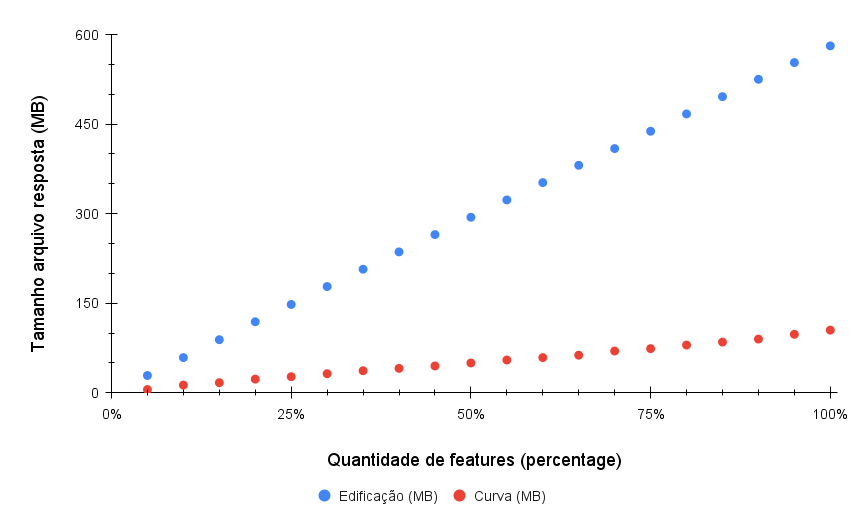
\includegraphics[width=0.8\textwidth]{img/chart.png}
\caption{Crescimento do tamanho do arquivo resposta por porcentagem de features requisitadas para os dois conjuntos de dados escolhidos que possuem mais de uma features}
\label{fig:comparesizes}
\end{figure}


\subsection{Processamento}

A avaliação será realizada sobre os resultados de execução de uma ferramenta de benchmarking HTTP configurada para realizar 50 requisições, sem concorrência, para cada coleção de features. O benchmark será realizado três vezes para cada amostra para garantir a confiabilidade dos tempos de execução obtidos na avaliação.

Para avaliar o efeito do número de features requisitadas e o efeito da abordagem, um Design Fatorial de dois níveis fserá utilizado, o que tornará possível diferenciar como cada fator interfere na performance da abordagem escolhida e estimar o erro exponencial. Para comparar o efeito entre as abordagens e estimar qual performa melhor, um Design Fatorial de um fator é utilizado, já que devemos comparar diversas alternativas de um único fator. A partir dos resultados, uma análise por regressão linear nos permite extrapolar ou interpolar sobre os tempos de resposta de ambas as abordagens e verificar quando uma abordagem prevalece sobre a outra. As técnicas de avaliação utilizadas até então estão disponíveis em \cite{bukh1992art}.

        %\chapter{Avaliação dos Resultados}\label{sec:resultados}
        %\input{chapters/resultados}
        %\chapter{Conclusão}\label{sec:conclusao}
        %% Discussão dos resultados à luz dos objetivos da dissertação
% Análise das implicações práticas e teóricas dos resultados obtidos
% Exploração das limitações do estudo e possíveis viéses

% Sumário dos principais pontos abordados na dissertação
% Resposta aos objetivos da pesquisa
% Contribuições do estudo para o campo de conhecimento em questão
% Sugestões para trabalhos futuros e direcionamentos adicionais de pesquisa
	
			
		%% Referências
%		\renewcommand\bibname{Referências} %% Trabalhos em português
		\renewcommand\bibname{References} %% Trabalhos em inglês
		\bibliographystyle{plain}
		\bibliography{referencias}
		
		\begin{apendices}
            \chapter{Levantamento entre Desenvolvedores}
            \label{appendix:survey_questions}
            \begin{table}[H]
\centering
\resizebox{\columnwidth}{!}{%
\begin{tabular}{ll}
\hline
\multicolumn{1}{c}{\textbf{Question}} &
  \multicolumn{1}{c}{\textbf{Answer Type}} \\ \hline
\multicolumn{2}{c}{FOSS4G Profile} \\ \hline
Reasons to join and to stay in FOSS4G Community &
  14 multiple options \\
Year of the first experience in FOSS4g Community &
  Year entry \\
Number of users in the biggest project you are involved &
  Ten (1) to One million (6) \\
Experience with the OGC API specifications &
  \begin{tabular}[c]{@{}l@{}}No experience (1) to\\ Have created a server(5)\end{tabular} \\
Experience with the OGC Web Service specifications &
  \begin{tabular}[c]{@{}l@{}}No experience (1) to \\ Have created a server (5)\end{tabular} \\ \hline
\multicolumn{2}{c}{Software Metrics} \\ \hline
\begin{tabular}[c]{@{}l@{}}How much do you agree with the following sentence about effort: \\ API compliant with OGC API requires less time and resources to\\ develop than OGC compliant Web Service.\end{tabular} &
  Likert-scale (agreement) \\
\begin{tabular}[c]{@{}l@{}}How much do you agree with the following sentence about performance:\\ API compliant with OGC API is more efficient and able to scale than OGC\\ compliant Web Service.\end{tabular} &
  Likert-scale (agreement) \\
\begin{tabular}[c]{@{}l@{}}How much do you agree with the following sentence about maintainability: \\ API compliant with OGC API is easier to maintain and extend with new \\ functionality than OGC compliant Web Service.\end{tabular} &
  Likert-scale (agreement) \\
\begin{tabular}[c]{@{}l@{}}How much do you agree with the following sentence about reliability:\\ API compliant with OGC API is more stable and has less risk of failure\\ compared to OGC compliant Web Service.\end{tabular} &
  Likert-scale (agreement) \\ \hline
\multicolumn{2}{c}{Future of the OGC API} \\ \hline
\begin{tabular}[c]{@{}l@{}}How much do you agree that the current technological approaches for \\ serving geospatial data on the Web meet the needs of the modern world?\end{tabular} &
  Likert-scale (agreement) \\
\begin{tabular}[c]{@{}l@{}}How much functionality gap do you think exists between OGC API and \\ OGC Web Service?\end{tabular} &
  Likert-scale (intensity) \\
\begin{tabular}[c]{@{}l@{}}How long do you think it takes for the OGC API to consolidate and \\ dispense with the use of OWS as support?\end{tabular} &
  \begin{tabular}[c]{@{}l@{}}Its already consolidated (1) \\ to Four years+ (5)\end{tabular} \\
\begin{tabular}[c]{@{}l@{}}Would you like to add comments about your personal perception \\ of the OGC API?\end{tabular} &
  Open-Ended
\end{tabular}%
}
\caption{Questionário sobre a Percepção e Avaliação dos desenvolvedores de Software Livre e Aberto sobre a OGC API}
\label{tab:survey-questions}
\end{table}
            \chapter{Resultado da Pesquisa Qualitativa}
            \label{appendix:results_qual}
            This section presents an overview of the survey results. The survey was sent to 60 developers, getting a response from 25\% of them, totaling 15 answers.

\section{Developers Profile}

The \ref{fig:reasons} image shows the percentage of developers who identify with the reasons to join and stay in Free and Open Source for Geospatial Community.

 Most of them report joining the community to share knowledge and skills, learn and develop new skills, participate in the FOSS scene, participate in a new form of cooperation and improve products of other developers. In the \ref{fig:year} we can see that the year of the first experience in FOSS is well distributed along the years, starting from 1992 and ending in 2020. This reflects the fact that it is a solid and very closed community.

\begin{figure}[]
     \centering
     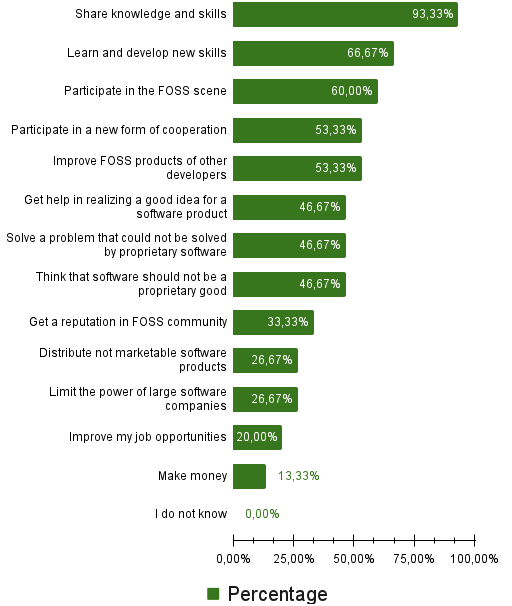
\includegraphics[scale=0.7]{img/reaons.png}
     \caption{Reasons to join and to stay in Free and Open Source Software (FOSS) for Geospatial Community}
     \label{fig:reasons}
\end{figure}
 
\begin{figure}[]
     \centering
     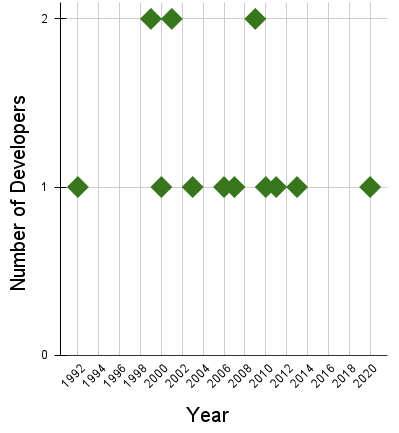
\includegraphics[scale=0.7]{img/year.png}
     \caption{Year of the first experience in Free and Open Source Software for Geospatial Community}
     \label{fig:year}
\end{figure}


\begin{figure}[]
     \centering
     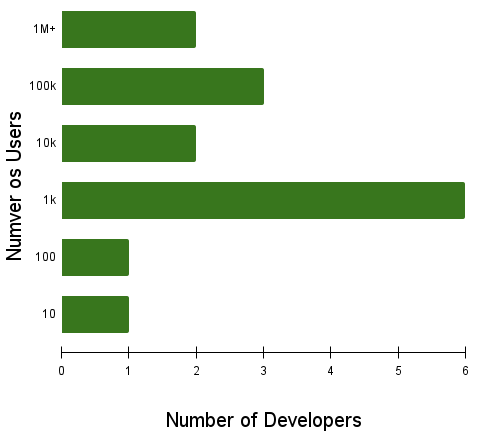
\includegraphics[scale=0.8]{img/users.png}
     \caption{ Number of users in the biggest project you are involved}
     \label{fig:users}
\end{figure}
In the figure \ref{fig:users} it is possible to observe that most of the developers are involved in big projects, and the responding developers who have projects with more than 100,000 users started in the FOSS community until 2003.

One of the biggest concerns when choosing respondents for the survey was choosing experienced users in the implementation of at least one of the proposed approaches. The results of the figure \ref{fig:apixp} show that 80\% of the respondents have some familiarity with the implementation or use of an API based on some specification of the OGC API. 

For the legacy service (figure \ref{fig:wsxp}), OGC Web Service, more than 93\% of respondents were familiar with it, with 86.7\% being developers who have already implemented a Web Service client or server. 

\begin{figure}[H]
     \centering
     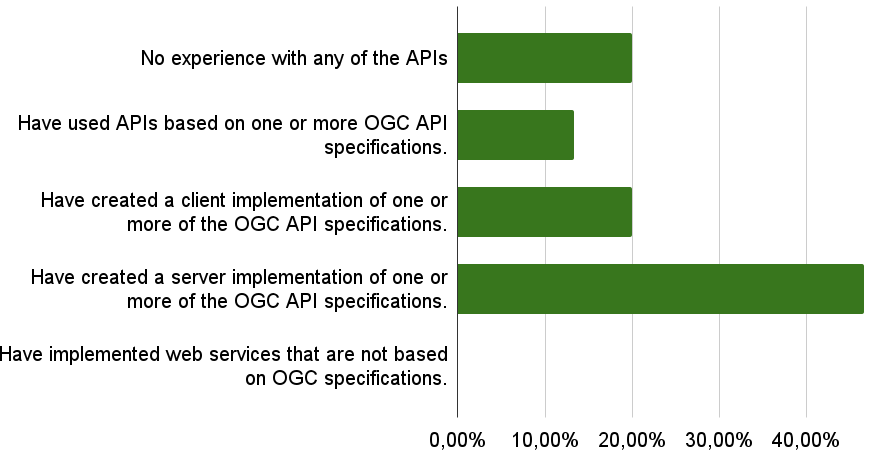
\includegraphics[scale=0.5]{img/apixp.png}
     \caption{Experience with the OGC API specifications }
     \label{fig:apixp}
\end{figure}

\begin{figure}[H]
     \centering
     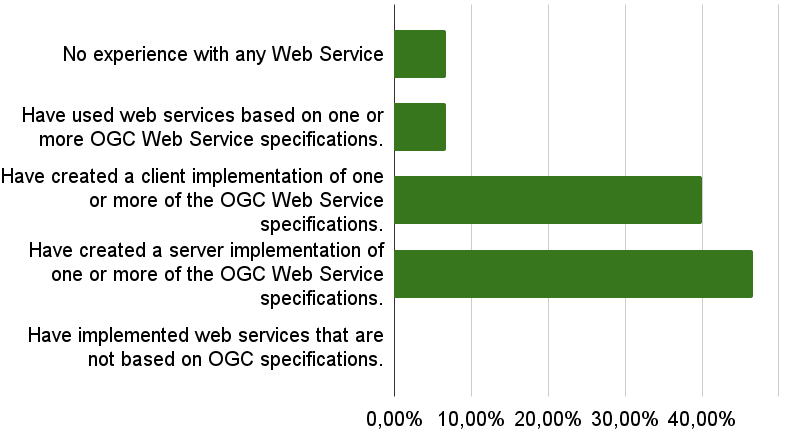
\includegraphics[scale=0.55]{img/wsxp.png}
     \caption{Experience with the OGC Web Service specifications }
     \label{fig:wsxp}
\end{figure}

The results of this section show the maturity of the public selected to respond to the survey. This guarantees less bias from users who are not familiar with the OGC API or OGC Web Services and are not well-educated on what is the OGC API.

\section{Software Evaluation}

For effort evaluation (figure \ref{fig:effort}) 66.63\% of participants answered "strongly agree" and "agree" that OGC API requires less resource and time to develop. Only one participant, with experience in creating a server implementation of both API and Web Service, disagreed with this statement.

\begin{figure}[H]
     \centering
     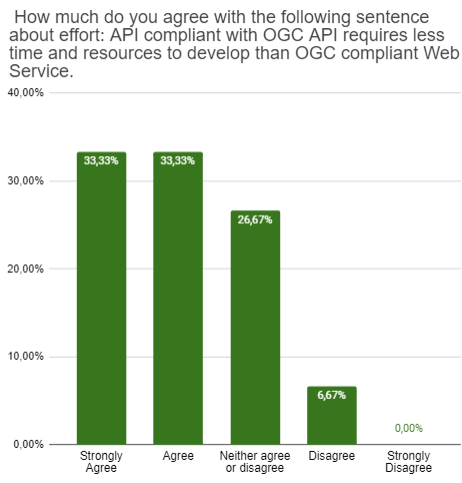
\includegraphics[scale=0.9]{img/effort.png}
     \caption{Effort Comparison}
     \label{fig:effort}
\end{figure}


\begin{figure}[H]
     \centering
     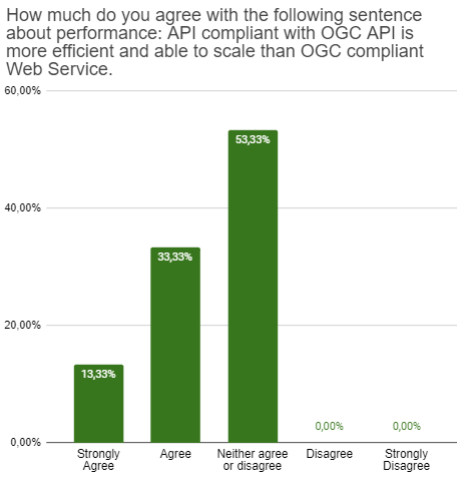
\includegraphics[scale=0.9]{img/performance.png}
     \caption{Performance Comparison}
     \label{fig:performance}
\end{figure}

\begin{figure}[H]
     \centering
     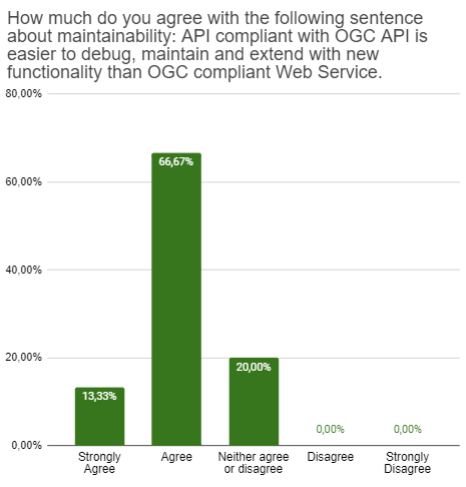
\includegraphics[scale=0.8]{img/maintain.png}
     \caption{Maintainability Comparison}
     \label{fig:maintain}
\end{figure}

Participants responses (figure \ref{fig:performance}) indicate that no developer believes that the Web Service performs better, but more than 50\% of the participants answered "neither agree or disagree". 46.6\% of participants believe that the API approach is more efficient and able to scale than OGC compliant Web Service.


\begin{figure}[H]
     \centering
     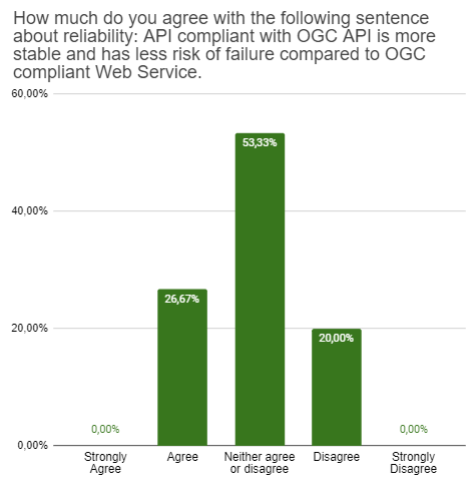
\includegraphics[scale=0.8]{img/reliability.png}
     \caption{Reliability Comparison}
     \label{fig:reliability}
\end{figure}

None of the participants believe that an OGC-compliant Web Service is easier to maintain than an API (figure \ref{fig:maintain}). 80\% of responses show that they believe API is easier to maintain, debug and extend functionality. Statement that maintains agreement with recent studies on the ease of implementing an API.


The developers demonstrated that there is no clear agreement on which approach has the highest reliability. Although the literature concludes that the REST approach is missing its own security model \cite{tihomirovs2016comparison}, the survey indicates that the tendency of participants is to believe that the API is more secure (figure \ref{fig:reliability}).


\section{Future of OGC API}


\begin{figure}[H]
     \centering
     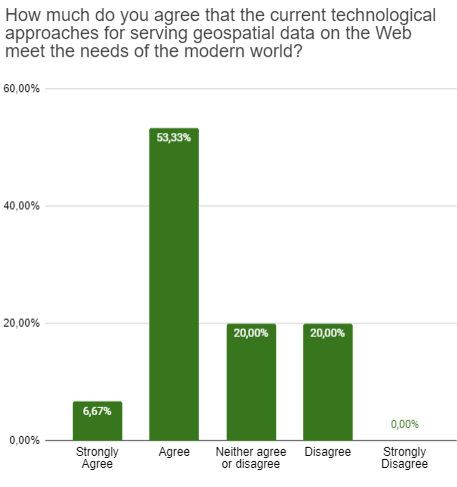
\includegraphics[scale=0.8]{img/modern.png}
     \caption{}
     \label{fig:modern}
\end{figure}

Most participants, around 60\%, believe that the current technological approaches for serving geospatial data on the Web meet the needs of the modern world, only 20\% disagree (figure \ref{fig:modern}).

The OGC API family has several standards for different types of spatial data and their metadata. From the 14 standards, five types were chosen that have not yet completed all the standards documents. Features is the most used standard, consequently it had the most applicable responses, the participants' opinion is distributed between minor, moderate and major gap. A major gap was also observed in the standard of Environmental Data Retrieval (EDR) and Records (a metadata standard). The 3D Volumes pattern got 70\% "not applicable" responses showing that developers are not yet widely using the standard.


\begin{figure}[H]
     \centering
     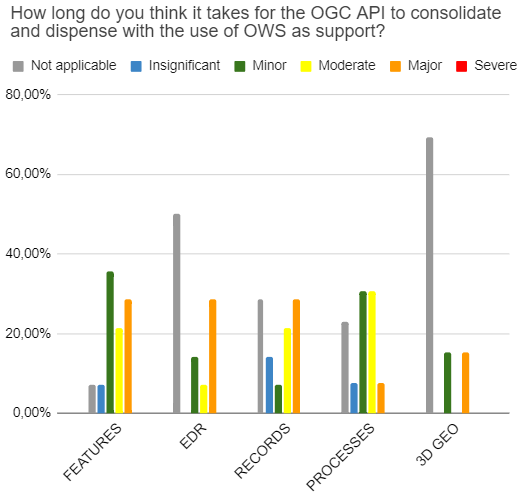
\includegraphics[scale=0.84]{img/gap.png}
     \caption{
     Functionality Gap between the standards families}
     \label{fig:gap}
\end{figure}



\begin{figure}[H]
     \centering
     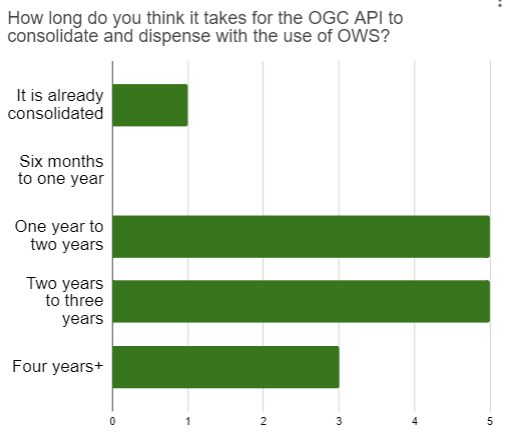
\includegraphics[scale=0.7]{img/consolidate.png}
     \caption{Time to OGC API to consolidate}
     \label{fig:consolidate}
\end{figure}

As can be seen in figure \ref{fig:consolidate}, only one person stated that the OGC API is already consolidated, no participant believes that the OGC API will be consolidated within a year. The other 92\% believe that it will be consolidated in at least one year.

                \chapter{Resultado da Pesquisa Quantitativa}    \label{appendix:results_quant}
            
In this section, we perform experiments and evaluate the response time of OGC-compliant API and Web services, considering the parameters and data described in the previous section.

\section{Experimental Setup}

To discuss the parameters, the work was divided into three main steps, varying the parameters in order to determine the effect of each factor on the performance of the approach. Two alternatives were analyzed for each parameter, so their effects can be compared using Two Level Factorial Design, while isolating an estimation of the experimental error. Performance is assessed in relation to data size, and a linear regression model is used in the analysis of several subset alternatives.

The first step is to run the experiments in an environment that processes other allocated tasks in parallel. The workload obtained in compliance with the OGC WFS was generated from the execution of requests for subsets of XML data to GeoServer \footnote{GeoServer: \url{https://geoserver.org/}} containerized and orchestrated with Docker Swarm served with Nginx. The workload of an OGC API application was obtained by requesting subsets of GeoJSON data to a pygeoapi \footnote{pygeoapi: \url{https://pygeoapi.io/}} implementation served with Flask Web Server Gateway Interface (WSGI) and data provided via OGR, from the Geospatial Data Abstraction Library (GDAL)\footnote{GDAL: \url{https://gdal.org/}}. GDAL supports a wide range of spatial file formats to be published using pygeoapi. In this workload, we used a shapefile to make data available.

The second step consists of running the experiments in order to compare the performance of services in an isolated environment and expand the workload. The load obtained with OGC WFS consists of requests from the same dataset in XML format. GeoServer is implemented with Apache and without dockerization to allow a fair comparison with the OGC API workload, which is provided by pygeoapi served with Apache and querying a shapefile with GDAL support.% At this stage, a workload of a GeoServer adaptation was also obtained to serve the data via API, this adaptation was made using the OGC API Extension plugin \footnote{OGC API Extension for Geoserver: https://docs.geoserver.org/latest/en/user/community/ogc-api/index.html}.

The third step aims to compare the approaches with two implementations that connect directly to the same database, therefore comparing the GeoServer Web service producing XML data with the pygeoapi API with the same data provided in two ways: querying the shapefile using GDAL, and querying the same database to which GeoServer is connected, without concurrency.

To ensure a fair comparison of services, sorting by feature ID was configured in both systems and the ``beautify'' output function was disabled in the requests in both systems. With this, we ensured that the resulting feature sets are equivalent. Cache settings were disabled.

We ran the isolated environment experiments in an AMD Ryzen 7 5800H with 16GB RAM and 512GB SSD, and the non-isolated environment experiments in an Intel Xeon(R) Silver 4215 with 128GB RAM and 4TB HD.

\section{Execution Environment Experiments}

Table \ref{tab:limiteenvironment} presents the benchmark results for the request of the dataset with only one feature for four experiments:

\begin{enumerate}
    \item \textbf{API on an Isolated Environment using GDAL}. OGC API Features implementation using pygeoapi deployed in an isolated environment using Apache and without concurrency tasks. The dataset is read from a shapefile using the GDAL library.
    \item \textbf{Web Service on an Isolated Environment connected to database}. OGC WFS implementation using GeoServer deployed in an environment without other allocated tasks using Apache.
    \item \textbf{API on a Non-Isolated Environment using GDAL}. OGC API Features implementation using pygeoapi deployed in an environment with other allocated tasks. The dataset is read from a shapefile using the GDAL library.
    \item \textbf{Web Service on a Non-Isolated Environment connected to database}. OGC WFS implementation using GeoServer connected to a database in an environment with other allocated tasks. The application consists of multiple services with orchestrated deploy using Docker Swarm.
%    \item \textbf{Server with OGC API Extension on Isolated Environment connected to database}. GeoServer with the OGC API Extension plugin connected to a database in an environment using Apache.
\end{enumerate}
%atualizado
\begin{table}[H]
\small
\centering
\caption{Minas Gerais state boundaries data -- Request Response Time Varying Environment}
\label{tab:limiteenvironment}
\begin{tabular}{|c|c|c|c|c|}
\cline{1-4}
 Experiment & Average (ms) & \begin{tabular}[c]{@{}c@{}}Standard \\ Deviation (ms)\end{tabular} & \begin{tabular}[c]{@{}c@{}}99,99\% \\ Confidence Interval\end{tabular} \\ \hline
\multicolumn{1}{|c|}{API on an Isolated Environment}     & 1396 & 341 & {[}1240,1560{]}  \\ \hline
\multicolumn{1}{|c|}{Web Service on an Isolated Environment}         & 147  & 45  & {[}126, 168{]}   \\ \hline
\multicolumn{1}{|c|}{API on a Non-Isolated Environment} & 1528 & 445 & {[}1320, 1740{]} \\ \hline
Web Service on a Non-Isolated Environment & 165  & 41  & \multicolumn{1}{c|}{{[}146, 184{]}}   \\ \hline

\end{tabular}
\end{table}

We observe from the execution of the experiments that the API approach using a shapefile as data source resulted in an average response time of 1528ms for the implementation in an environment with other tasks allocated and an average time of 1396ms for an isolated environment. 
\newpage
However, when analyzing the confidence interval we observed, with 99.9\% confidence, that the response time performance is not significantly different in the two approaches. The same happens for the Web service approach, in which the average response time in the non-isolated environment is 165ms and 147ms in an isolated environment. We can also state, with 99.9\% confidence, that the response times of the approaches are not significantly different. 

Therefore, we conclude that the runtime setup and deployment environmental factors do not significantly affect the response times for the spatial data request. We can also say, with 99.9\% confidence, that the Web service approach is superior to the API when directly querying the Shapefile, contradicting previous research \cite{mumbaikar2013web} that shows that the Web service approach has lower performance than REST APIs.

To determine the effect of the other two parameters, we performed a Two Level Factorial Design, in which each factor was modeled to have two levels, so that variable A represents the service type approach (OGC API = 1 and WFS = -1)and variable B represents the execution environment (Isolated Environment = 1 and Non Isolated Environment = -1).


 The Two Level Factorial Design analysis is represented in Table \ref{tab:twofactorialdesignLimite}.
 From the coefficients we found, we know that the execution environment is responsible for only 0.33\% of the variation, while the type of service is responsible for 99.48\% of the total variation. The interaction between them accounts for 0.19\% of the response time variation.

%atualizado nao consigo visualizar como melhorar a legibiliadde da parte de AB que é a interação entre os dois fatores, acredito que nao aplicaria a observação do review

\begin{table}[H]
\centering
\caption{Sign Table of Calculating Effect of Standard Approach and Environment}
\label{tab:twofactorialdesignLimite}
\begin{tabular}{ccccc}
\hline
I    & A    & B     & AB    & y       \\ \hline
1    & WFS   & Non Isolated    & 1     & 165     \\
1    & API     & Non Isolated    & -1    & 1528    \\
1    & WFS   & Isolated     & -1    & 147     \\
1    & API    & Isolated     & 1    & 1396     \\
3236 & 2612 & -150  & -114  & Total   \\
809  & 653  & -37.5 & -28.5 & Total/4 \\ \hline
\end{tabular}
\end{table}

\begin{table}[H]
\centering
\caption{Sign Table of Calculating Effect of Standard Approach and Environment}
\label{tab:twofactorialdesignLimite}
\begin{tabular}{ccccc}
\hline
I    & A    & B     & AB    & y       \\ \hline
1    & -1   & -1    & 1     & 165     \\
1    & 1    & -1    & -1    & 1528    \\
1    & -1   & 1     & -1    & 147     \\
1    & 1   & 1     & 1    & 1396     \\
3236 & 2612 & -150  & -114  & Total   \\
809  & 653  & -37.5 & -28.5 & Total/4 \\ \hline
\end{tabular}
\end{table}

\section{Data Storage Experiments}

The dataset chosen to carry out the experiments that compare the response time of the GeoServer Web service vs pygeoapi directly querying a PostGIS database vs pygeoapi querying a shapefile with the GDAL/OGR library was the one containing buildings in Belo Horizonte, which has 740,765 features. Benchmarking was performed in the three approaches, and the average response time is depicted in Figure \ref{fig:timeperfeature_dispersaoedificacao}. For a small subset of features, the Web service has a superior response time performance, and the API querying the database directly is slower than the other two approaches. After a certain number of features in the query, the API querying the database becomes faster.

\begin{figure}[H]
\centering
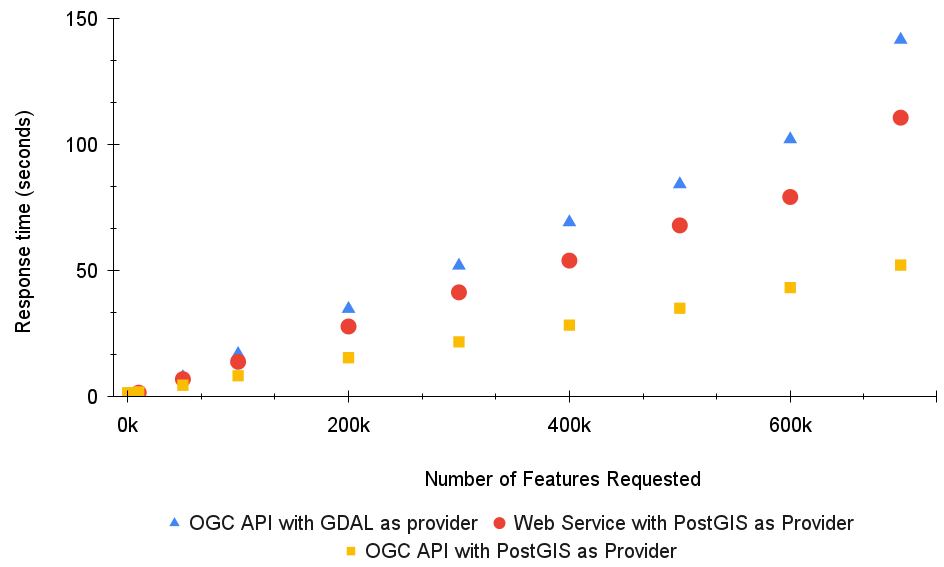
\includegraphics[width=0.8\textwidth]{img/dispersaoedificacao.png}
\caption{Average response time per maxFeatures requested for Edificacao}
\label{fig:timeperfeature_dispersaoedificacao}
\end{figure}

One-factor design can be used to compare a single factor with multiple alternatives and be able to compute the effect of each alternative. The table \ref{tab:onefactor} shows the three average response times for requests for 100,000 spatial data features obtained from three executions of the experiment for each approach. Computing the one-factor design we found that an average service requires 12955ms to respond to the chosen 100 thousand features of the dataset, corresponding to a 71M file. The API with GDAL as provider requires 7225.28ms more than the average service, a Web service requires 648.88ms more than the average service and the API querying the database requires 4874.77ms less than the average service. From the Analysis of Variance (ANOVA) we verified with 95\% confidence that the approach factor variation is significant.

\begin{table}[H]
\centering
\caption{Average Request Response for Three Executions }
\label{tab:onefactor}
\begin{tabular}{cc|c|c}
\cline{2-4}
\multicolumn{1}{l|}{}                                     & y                   & Mean     & \multicolumn{1}{c|}{Effect}  \\ \hline
\multicolumn{1}{|c|}{OGC API with GDAL as provider}       & (17424,16912,17209) & 17181,67 & \multicolumn{1}{c|}{4225,88} \\ \hline
\multicolumn{1}{|c|}{WFS with PostGIS as Provider} & (13793,13327,13694) & 13604,67 & \multicolumn{1}{c|}{648,88} \\ \hline
\multicolumn{1}{|c|}{OGC API with PostGIS as Provider} & (7962,8041,8240)    & 8081,00  & \multicolumn{1}{c|}{-4874,77}  \\ \hline
\multicolumn{1}{l}{}                                      & Total mean          & 12955,77 & \multicolumn{1}{l}{}         \\ \cline{3-3}
\end{tabular}
\end{table}

 From the linear regression model of the three alternatives discussed, which fits more than 98\% of the sample, %% ?? which achieved a correlation coefficient of 0.98 ? o coeficiente de determinação (R²) é de 98% no minimo pros tres, o quao bem o modelo prediz o tempo de resposta
 we observe the points of intersection where one approach becomes superior to the other. In Figure \ref{fig:comparetodos}, we can see that, from a dataset with 740,765 features, the API querying a Shapefile is superior to all other approaches up to 18,069 features, which corresponds to a 13MB file and 2.4\% of the requested dataset. Although initially the API querying the data in the database presents a significantly lower response time than the other approaches, the slope of its linear regression model is much smaller than that of the other approaches, so we can observe from the graph of the figure \ref{fig:comparetodos} that from 22,831 features requested onward, the response time of an API that directly queries the database is lower and grows more slowly than the other approaches.

\begin{figure}[H]
\centering
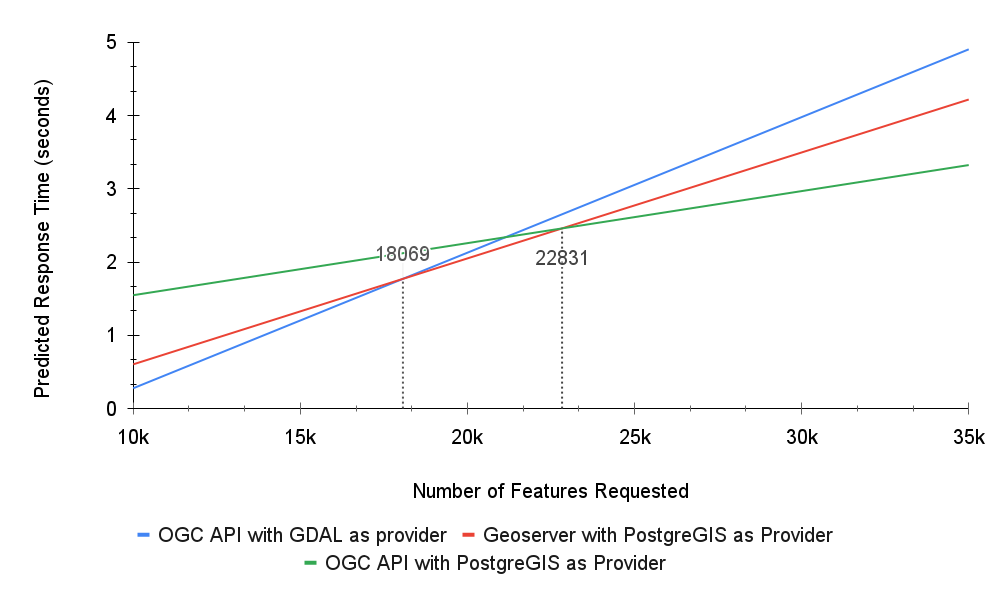
\includegraphics[width=0.9\textwidth]{img/comparetodos.png}
\caption{Linear regression for response time intersection}
\label{fig:comparetodos}
\end{figure}

\section{Data Type and Size Experiments}

To evaluate the impact of the variability in the size of the features and the type of spatial data geometry, we performed experiments to compare response times for varied workloads. 
%were performed that compare the file size and its response time for each fraction of each dataset. 
These experiments were performed using data storage in PostGIS for the API, using both large datasets. Figure \ref{fig:filesize} shows the file size increments for each requested fraction of the feature set for the two datasets, and Figure \ref{fig:timesize} shows the response time increase for the same fractions of the feature set.

For both approaches, a correlation coefficient above 99\% was calculated between the response time and the response size, indicating that as the response size increases, the response time increases linearly. Since both variables are related to the workload size, this result suggests that the workload size directly influences both the time and the response size.

\begin{figure}[H]
\centering
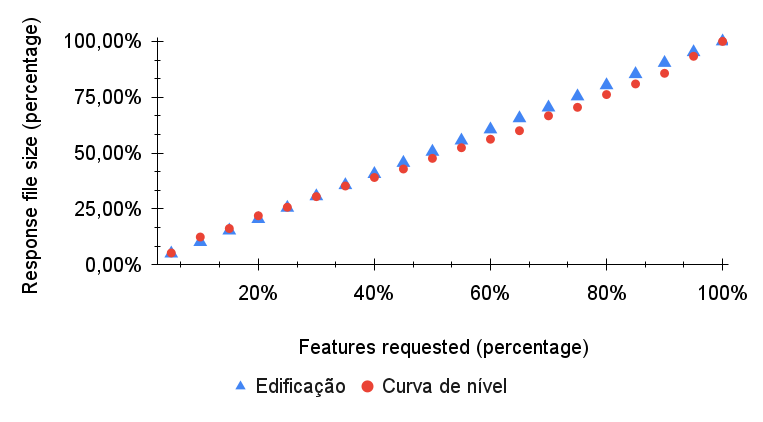
\includegraphics[width=0.7\textwidth]{img/comparesize.png}
\caption{Response file size per percentage of features requested for each dataset}
\label{fig:filesize}
\end{figure}

\begin{figure}[H]
\centering
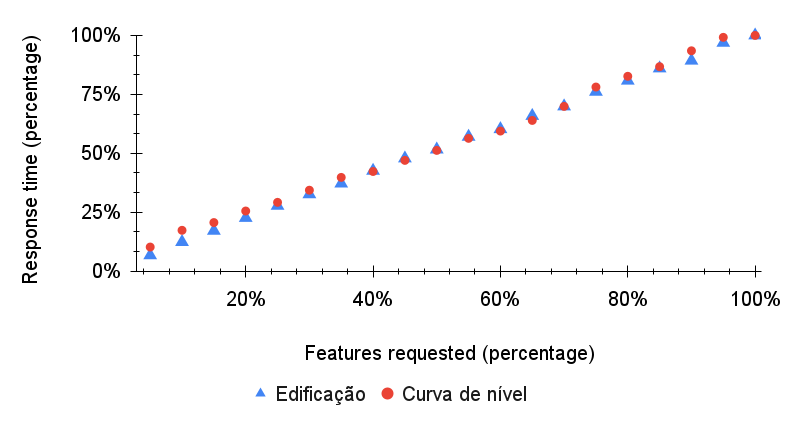
\includegraphics[width=0.7\textwidth]{img/comparetimeresponsecurvaedificacao.png}
\caption{Response time per percentage requested for each dataset}
\label{fig:timesize}
\end{figure}

		\end{apendices}
		
\end{document}
